% -*- mode: latex; -*- mustache tags:  
\documentclass[10pt,twoside,english]{_support/latex/sbabook/sbabook}
\let\wholebook=\relax

\usepackage{import}
\subimport{_support/latex/}{common.tex}

%=================================================================
% Debug packages for page layout and overfull lines
% Remove the showtrims document option before printing
\ifshowtrims
  \usepackage{showframe}
  \usepackage[color=magenta,width=5mm]{_support/latex/overcolored}
\fi


% =================================================================
\title{Learning Object-Oriented Programming, Design and TDD with Pharo}
\author{Stéphane Ducasse}
\series{The Pharo TextBook Collection}

\hypersetup{
  pdftitle = {Learning Object-Oriented Programming, Design and TDD with Pharo},
  pdfauthor = {Stéphane Ducasse},
  pdfkeywords = {Introduction, programming, design, testing, Pharo, Smalltalk}
}


% =================================================================
\begin{document}

% Title page and colophon on verso
\maketitle
\pagestyle{titlingpage}
\thispagestyle{titlingpage} % \pagestyle does not work on the first one…

\cleartoverso
{\small

  Copyright 2017 by Stéphane Ducasse.

  The contents of this book are protected under the Creative Commons
  Attribution-ShareAlike 3.0 Unported license.

  You are \textbf{free}:
  \begin{itemize}
  \item to \textbf{Share}: to copy, distribute and transmit the work,
  \item to \textbf{Remix}: to adapt the work,
  \end{itemize}

  Under the following conditions:
  \begin{description}
  \item[Attribution.] You must attribute the work in the manner specified by the
    author or licensor (but not in any way that suggests that they endorse you
    or your use of the work).
  \item[Share Alike.] If you alter, transform, or build upon this work, you may
    distribute the resulting work only under the same, similar or a compatible
    license.
  \end{description}

  For any reuse or distribution, you must make clear to others the
  license terms of this work. The best way to do this is with a link to
  this web page: \\
  \url{http://creativecommons.org/licenses/by-sa/3.0/}

  Any of the above conditions can be waived if you get permission from
  the copyright holder. Nothing in this license impairs or restricts the
  author's moral rights.

  \begin{center}
    
\includegraphics[width=0.2\textwidth]{_support/latex/sbabook/CreativeCommons-BY-SA.pdf}
  \end{center}

  Your fair dealing and other rights are in no way affected by the
  above. This is a human-readable summary of the Legal Code (the full
  license): \\
  \url{http://creativecommons.org/licenses/by-sa/3.0/legalcode}

  \vfill

  % Publication info would go here (publisher, ISBN, cover design…)
  Layout and typography based on the \textcode{sbabook} \LaTeX{} class by Damien
  Pollet.
}


\frontmatter
\pagestyle{plain}

\tableofcontents*
\clearpage\listoffigures

\mainmatter

\chapter{A little expression interpreter}\label{cha:expressions}
In this chapter you will build a small mathematical expression interpreter. For example you will be able to build an expression such as  (3 + 4) * 5 and then ask the interpreter to compute its value. You will revisit tests, classes, messages, methods and inheritance. 
You will also see an example of expression trees similar to the ones that are used to manipulate programs. For example, compilers and code refactorings as offered in Pharo and many modern IDEs are doing such manipulation with trees representing code. 
In addition, in the volume two of this book, we will extend this example to present the Visitor Design Pattern. 
\section{Starting with constant expression and a test}
We start with constant expression. A constant expression is an expression whose value is always the same, obviously.

Let us start by defining a test case class as follows: 

\begin{displaycode}{plain}
TestCase subclass: #EConstantTest
	instanceVariableNames: ''
	classVariableNames: ''
	package: 'Expressions'
\end{displaycode}

 We decided to define one test case class per expression class and this even if at the beginning the classes will not contain many tests. It is easier to define new tests and navigate them.
 
Let us write a first test making sure that when we get a value, sending it the \textcode{evaluate} message returns its value. 

\begin{displaycode}{plain}
EConstantTest >> testEvaluate 
	self assert: (EConstant new value: 5) evaluate equals: 5
\end{displaycode}

When you compile such a test method, the system should prompt you to get a class \textcode{EConstant} defined. 
Let the system drive you. Since we need to store the value of a constant expression, let us add an instance variable \textcode{value}
to the class definition. 

At the end you should have the following definition for the class \textcode{EConstant}.

\begin{displaycode}{plain}
Object subclass: #EConstant
	instanceVariableNames: 'value'
	classVariableNames: ''
	package: 'Expressions'
\end{displaycode}

We define the method \textcode{value:} to set the value of the instance variable \textcode{value}.
It is simply a method taking one argument and storing it in the \textcode{value} instance variable.

\begin{displaycode}{plain}
EConstant >> value: anInteger
	value := anInteger
\end{displaycode}

You should define the method \textcode{evaluate}: it should return the value of the constant. 

\begin{displaycode}{plain}
EConstant >> evaluate
	... Your code ...
\end{displaycode}

Your test should pass. 
\section{Negation}
Now we can start to work on expression negation. Let us write a test and for this define a new test case class named \textcode{ENegationTest}. 

\begin{displaycode}{plain}
TestCase subclass: #ENegationTest
	instanceVariableNames: ''
	classVariableNames: ''
	package: 'Expressions'
\end{displaycode}

The test \textcode{testEvaluate} shows that a negation applies to an expression (here a constant) and when we evalute we get the negated value of the constant. 

\begin{displaycode}{plain}
ENegationTest >> testEvaluate 
	self assert: (ENegation new expression: (EConstant new value: 5)) evaluate equals: -5
\end{displaycode}

Let us execute the test and let the system help us to define the class. A negation defines an instance variable to hold the expression that it negates.

\begin{displaycode}{plain}
Object subclass: #ENegation
	instanceVariableNames: 'expression'
	classVariableNames: ''
	package: 'Expressions'
\end{displaycode}

We define a setter method to be able to set the expression under negation.

\begin{displaycode}{plain}
ENegation >> expression: anExpression 
	expression := anExpression
\end{displaycode}

Now the \textcode{evaluate} method should request the evaluation of the expression and negate it. 
To negate a number the Pharo library proposes the message \textcode{negated}. 

\begin{displaycode}{plain}
ENegation >> evaluate
	... Your code ...
\end{displaycode}


\begin{figure}

\begin{center}
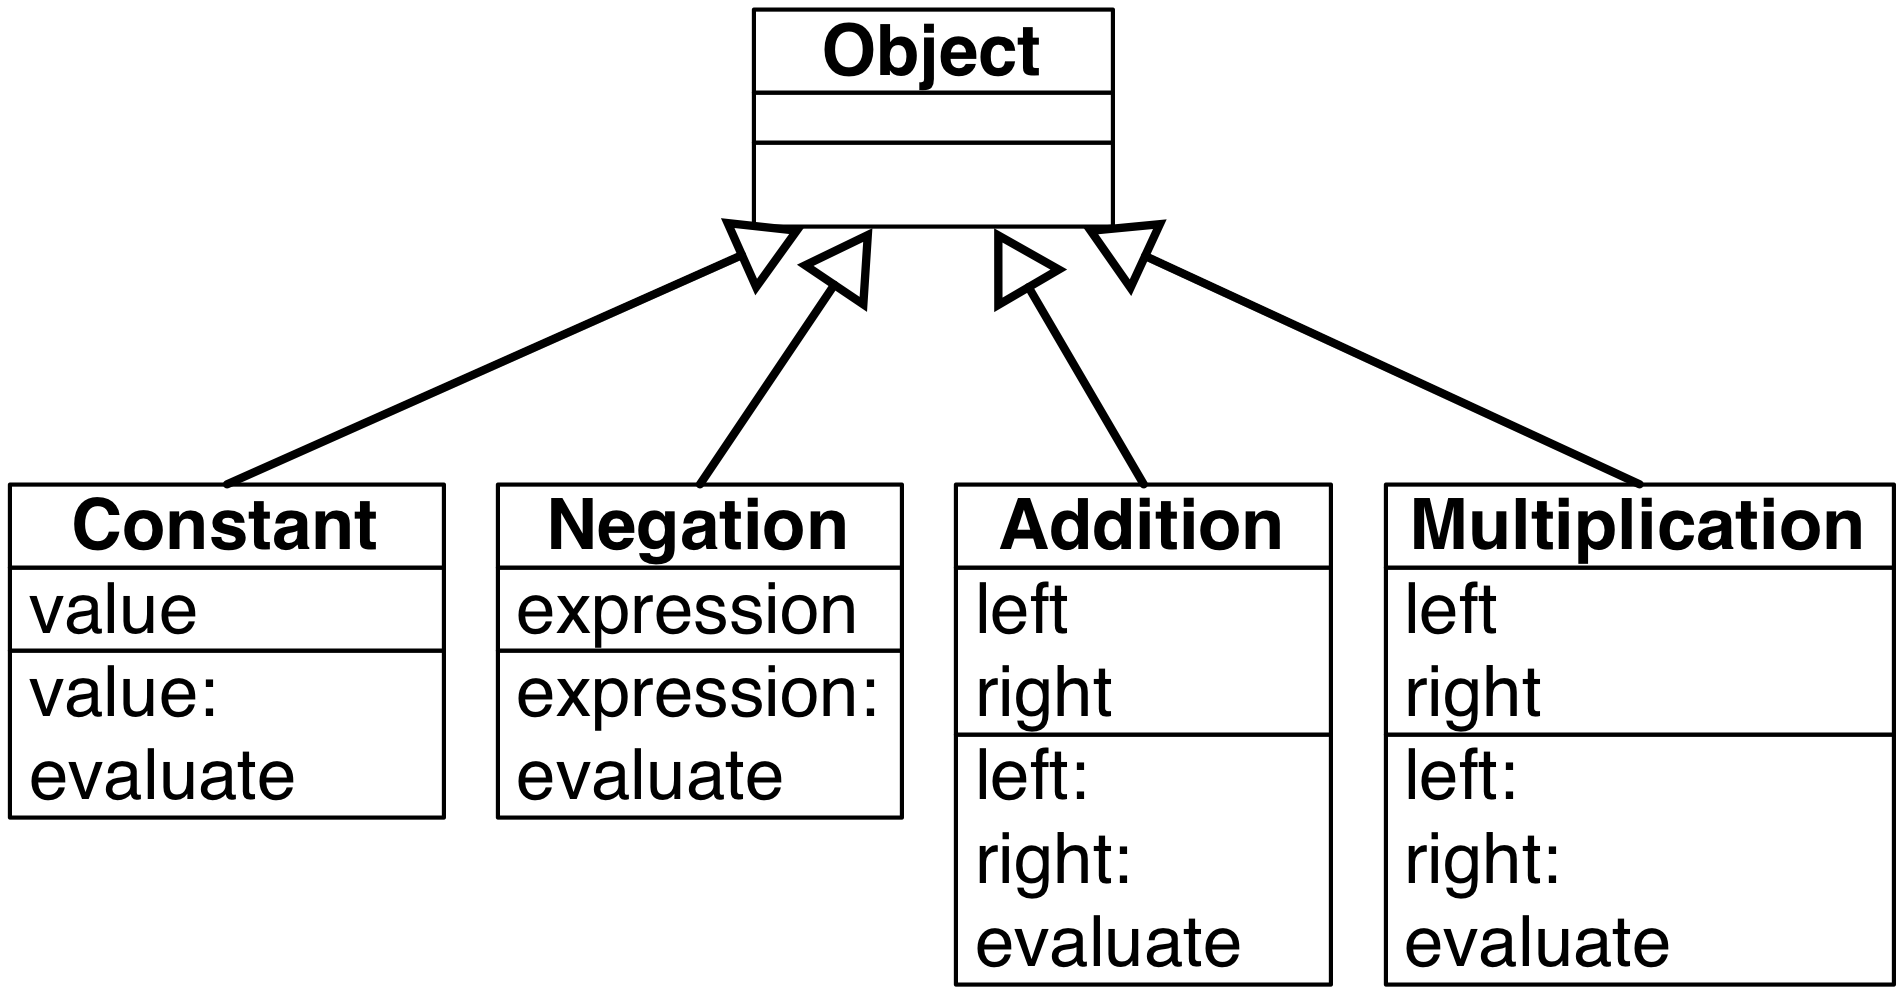
\includegraphics[width=0.7\textwidth]{/Users/ducasse/Workspace/FirstCircle/MyBooks/Bk-Writing/PharoBooks/LearningOOPWithPharoTrans/_result/pdf/Chapters/Expressions/figures/Expressions.png}\caption{A flat collection of classes (with a suspect duplication).\label{figExpression}}\end{center}
\end{figure}


Following the same principle, we will add expression addition and multiplication. Then we will make the system a bit more easy to manipulate and revisit its first design. 
\section{Adding expression addition}
To be able to do more than constant and negation we will add two extra expressions: addition and multiplication and after we will discuss about our approach and see how we can improve it.  

To add an expression that supports addition, we start to define a test case class and a simple test. 

\begin{displaycode}{plain}
TestCase subclass: #EAdditionTest
	instanceVariableNames: ''
	classVariableNames: ''
	package: 'Expressions'
\end{displaycode}

A simple test for addition is to make sure that we add correctly two constants. 

\begin{displaycode}{plain}
EAdditionTest >> testEvaluate
	| ep1 ep2 |
	ep1 := (EConstant new value: 5).
	ep2 := (EConstant new value: 3).
	self assert: (EAddition new right: ep1; left: ep2) evaluate equals: 8
\end{displaycode}

	
You should define the class \textcode{EAddition}: it has two instance variables for the two subexpressions it adds. 

\begin{displaycode}{plain}
EExpression subclass: #EAddition
	instanceVariableNames: 'left right'
	classVariableNames: ''
	package: 'Expressions'
\end{displaycode}

Define the two corresponding setter methods \textcode{right:} and \textcode{left:}. 

Now you can define the \textcode{evaluate} method for addition. 

\begin{displaycode}{plain}
EAddition >> evaluate
	... Your code ...
\end{displaycode}

	
To make sure that our implementation is correct we can also test that we can add negated expressions. 
It is always good to add tests that cover \textit{different} scenario. 
	

\begin{displaycode}{plain}
EAdditionTest >> testEvaluateWithNegation
	| ep1 ep2 |
	ep1 := ENegation new expression: (EConstant new value: 5).
	ep2 := (EConstant new value: 3).
	self assert: (EAddition new right: ep1; left: ep2) evaluate equals: -2
\end{displaycode}

	
	
\section{Multiplication}
We do the same for multiplication: create a test case class named \textcode{EMultiplicationTest}, a test, a new class \textcode{EMultiplication}, a couple of setter methods and finally a new \textcode{evaluate} method. Let us do it fast and without much comments. 

\begin{displaycode}{plain}
TestCase subclass: #EMultiplicationTest
	instanceVariableNames: ''
	classVariableNames: ''
	package: 'Expressions'
\end{displaycode}

\begin{displaycode}{plain}
EMultiplicationTest >> testEvaluate
	| ep1 ep2 |
	ep1 := (EConstant new value: 5).
	ep2 := (EConstant new value: 3).
	self assert: (EMultiplication new right: ep1; left: ep2) evaluate equals: 15
\end{displaycode}

\begin{displaycode}{plain}
Object subclass: #EMultiplication
	instanceVariableNames: 'left right'
	classVariableNames: ''
	package: 'Expressions'
\end{displaycode}

\begin{displaycode}{plain}
EMultiplication >> right: anExpression
	right := anExpression
\end{displaycode}

\begin{displaycode}{plain}
EMultiplication >> left: anExpression
	left := anExpression
\end{displaycode}

\begin{displaycode}{plain}
EMultiplication >> evaluate
	... Your code ...
\end{displaycode}
\section{Stepping back }
It is interesting to look at what we built so far. We have a group of classes whose instances can be combined to create complex expressions. Each expression is in fact a tree of subexpressions as shown in Figure \ref{fig:ExpressionTrees}. The figure shows two main trees: one  for the constant expression \textcode{5} and one for the expression \textcode{-5 + 3}. Note that the diagram represents the number 5 as an object because in Pharo even small integers are objects in the same way the instances of \textcode{EConstant} are objects. 


\begin{figure}

\begin{center}
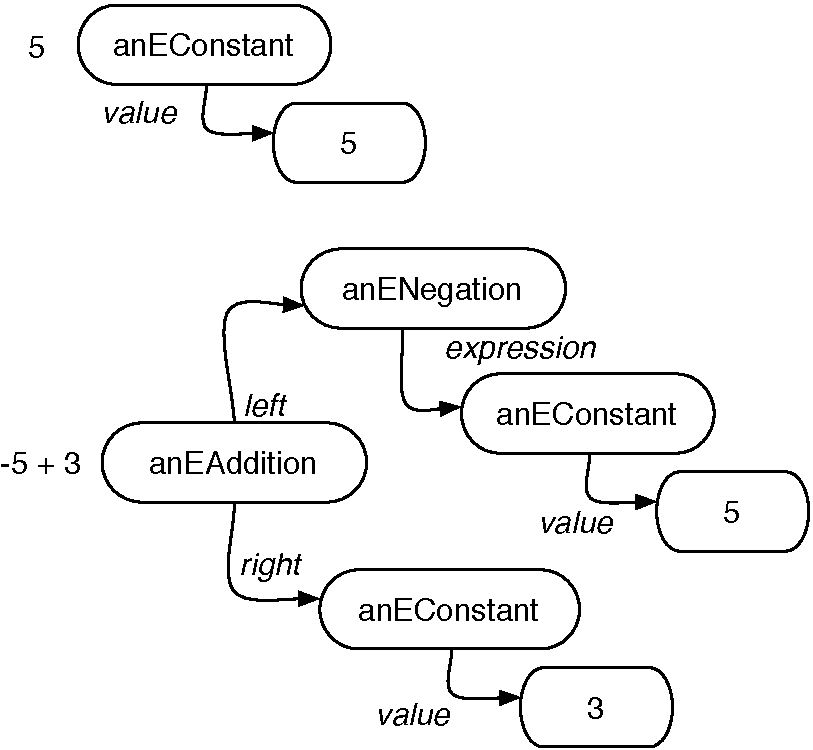
\includegraphics[width=0.6\textwidth]{/Users/ducasse/Workspace/FirstCircle/MyBooks/Bk-Writing/PharoBooks/LearningOOPWithPharoTrans/_result/pdf/Chapters/Expressions/figures/ExpressionTrees.pdf}\caption{Expressions are composed of trees.\label{fig:ExpressionTrees}}\end{center}
\end{figure}

\subsection{Messages and methods}
The implementation of the \textcode{evaluate} message is worth discussing. What we see is that \textit{different} classes understand the same message but execute different methods as shown in Figure \ref{figExpressionEvaluate}.

\begin{important}
A message represents an intent: it represents \textit{what} should be done. A method represents a specification of \textit{how} something should be executed.
\end{important}

What we see is that sending a message \textcode{evaluate} to an expression is making a choice among the different implementations of the message. This point is central to object-oriented programming. 

\begin{important}
Sending a message is making a choice among all the methods with the same name. 
\end{important}
\subsection{About common superclass}
So far we did not see the need to have an inheritance hierarchy because there is not much to share or reuse. Now adding a common superclass would be useful to convey to the reader of the code or a future extender of the library that such concepts are related and are different variations of expression. 


\begin{figure}

\begin{center}
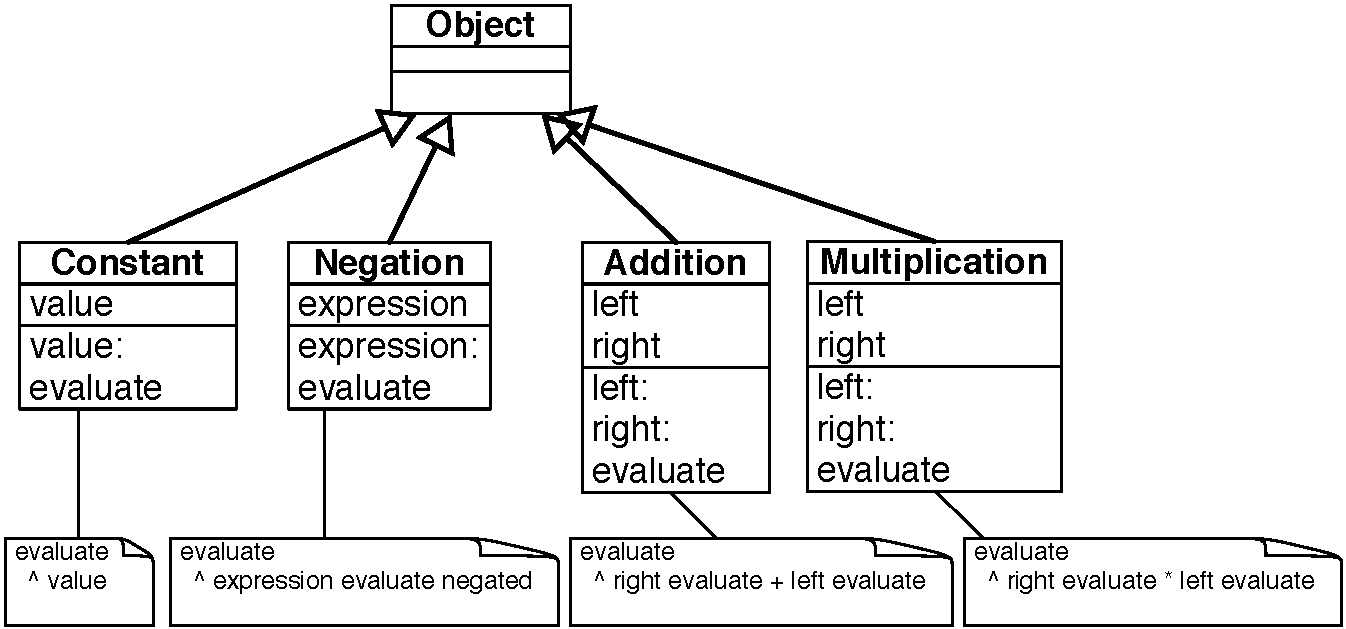
\includegraphics[width=0.8\textwidth]{/Users/ducasse/Workspace/FirstCircle/MyBooks/Bk-Writing/PharoBooks/LearningOOPWithPharoTrans/_result/pdf/Chapters/Expressions/figures/ExpressionsEvaluate.pdf}\caption{Evaluation: one message and multiple method implementations.\label{figExpressionEvaluate}}\end{center}
\end{figure}

\subsection{Design corner: About addition and multiplication model }
We could have just one class called for example BinaryOperation and it can have an operator and this operator will be either 
the addition or multiplication. This solution can work and as usual having a working program does not mean that its design is any good. 

In particular having a single class would force us to start to write conditional based on the operator as follows

\begin{displaycode}{plain}
BinaryExpression >> evaluate
	operator = #+ 
		ifTrue: [ left evaluate + right evaluate ] 
		ifFalse: [ left evaluate * right evaluate]
\end{displaycode}

There are ways in Pharo to make such code more compact but we do not want to use it at this stage. For the interested reader, look for the message \textcode{perform:} that can execute a method based on its name. 

This is annoying because the execution engine itself is made to select methods for us so we want to avoid to bypass it using explicit condition. In addition when we will add power, division, subtraction we will have to have more cases in our condition making the code less
readable and more fragile. 

As we will see as a general message in this book, sending a message is making a choice between different implementations. 
Now to be able to choose we should have different implementations and this implies having different classes. 

\begin{important}
Classes represent choices whose methods can be selected in reaction to a message. Having many little classes is better than few large ones.
\end{important}

What we could do is to introduce a common superclass between \textcode{EAddition} and \textcode{EMultiplication} but keep the two subclasses. We will probably do it in the future
\section{Negated as a message}
Negating an expression is expressed in a verbose way. We have to create explicitly each time an instance of the class \textcode{ENegation} as shown in the following snippet. 

\begin{displaycode}{plain}
ENegation new expression: (EConstant new value: 5)
\end{displaycode}

We propose to define a message \textcode{negated} on the expressions themselves that will create such instance of \textcode{ENegation}.
With this new message, the previous expression can be reduced too. 

\begin{displaycode}{plain}
(EConstant new value: 5) negated
\end{displaycode}
\subsection{negated message for constants}
Let us write a test to make sure that we capture well what we want to get. 

\begin{displaycode}{plain}
EConstantTest >> testNegated
	self assert: (EConstant new value: 6) negated evaluate equals: -6
\end{displaycode}

And now we can simply implement it as follows: 

\begin{displaycode}{plain}
EConstant >> negated
	^ ENegation new expression: self
\end{displaycode}
\subsection{negated message for negations}
\begin{displaycode}{plain}
ENegationTest >> testNegationNegated
	self assert: (EConstant new value: 6) negated negated evaluate equals: 6
\end{displaycode}

\begin{displaycode}{plain}
ENegation >> negated
	^ ENegation new expression: self
\end{displaycode}

This definition is not the best we can do since in general it is a bad practice to hardcode the class usage inside the class. A better definition would be 

\begin{displaycode}{plain}
ENegation >> negated
	^ self class new expression: self
\end{displaycode}

But for now we keep the first one for the sake of simplicity
\subsection{negated message for additions}
We proceed similarly for additions. 

\begin{displaycode}{plain}
EEAdditionTest >> testNegated
	| ep1 ep2 |
	ep1 := EConstant new value: 5.
	ep2 := EConstant new value: 3.
	self assert: (EAddition new right: ep1; left: ep2) negated evaluate equals: -8
\end{displaycode}

\begin{displaycode}{plain}
EAddition >> negated
	Your code
\end{displaycode}
\subsection{negated message for multiplications}
We proceed similarly for multiplications. 

\begin{displaycode}{plain}
EMultiplicationTest >> testEvaluateNegated
	| ep1 ep2 |
	ep1 := EConstant new value: 5.
	ep2 := EConstant new value: 3.
	self assert: (EMultiplication new right: ep1; left: ep2) negated evaluate equals: -15
\end{displaycode}

\begin{displaycode}{plain}
EMultiplication >> negated
	... Your code ...
\end{displaycode}

Now all your tests should pass. And it is a good moment to save your package. 
\section{Annoying repetition}
Let us step back and look at what we have. We have a working situation but again object-oriented design is to bring the code to a better level. 

Similarly to the situation of the \textcode{evaluate} message and methods we see that the functionality of \textcode{negated} is distributed over 
different classes. Now what is annoying is that we repeat the exact \textit{same} code over and over and this is not good (see Figure \ref{fig:ExpressionsNegatedRepeated}). 
This is not good because if tomorrow we want to change the behavior of negation we will have to change it four times while 
in fact one time should be enough. 


\begin{figure}

\begin{center}
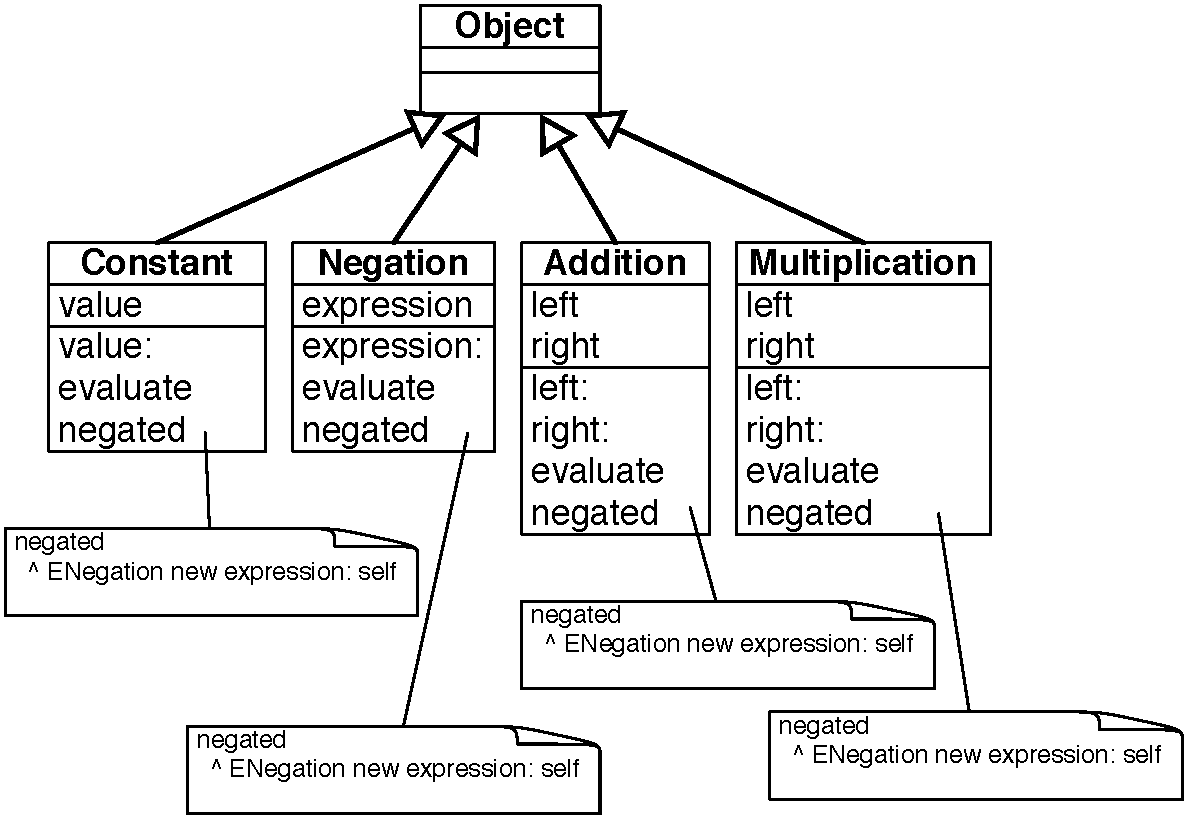
\includegraphics[width=0.7\textwidth]{/Users/ducasse/Workspace/FirstCircle/MyBooks/Bk-Writing/PharoBooks/LearningOOPWithPharoTrans/_result/pdf/Chapters/Expressions/figures/ExpressionsNegatedRepeated.pdf}\caption{Code repetition is a bad smell.\label{fig:ExpressionsNegatedRepeated}}\end{center}
\end{figure}


What are the solutions?

\begin{itemize}
\item We could define another class \textcode{Negator} that would do the job and each current classes would delegate to it. But it does not really solve our problem since we will have to duplicate all the message sends to call \textcode{Negator} instances. 
\item If we  define the method \textcode{negated} in the superclass (\textcode{Object}) we only need one definition and it will work. Indeed, when we send the message \textcode{negated} to an instance of \textcode{EConstant} or \textcode{EAddition} the system will not find it locally but in the superclass \textcode{Object}. So no need to define it four times but only one in class \textcode{Object}. This solution is nice because it reduces the number of  similar definitions of the method \textcode{negated} but it is not good because even if in Pharo we can add methods to the class \textcode{Object} this is not a good practice. \textcode{Object} is a class shared by the entire system so we should take care not to add behavior only making sense for a single application. 
\item The solution is to introduce a new superclass between our classes and the class \textcode{Object}. It will have the same property than the solution with \textcode{Object} but without polluting it (see Figure \ref{figExpressionHierar}). This is what we do in the next section. 
\end{itemize}
\section{Introducing Expression class}

\begin{figure}

\begin{center}
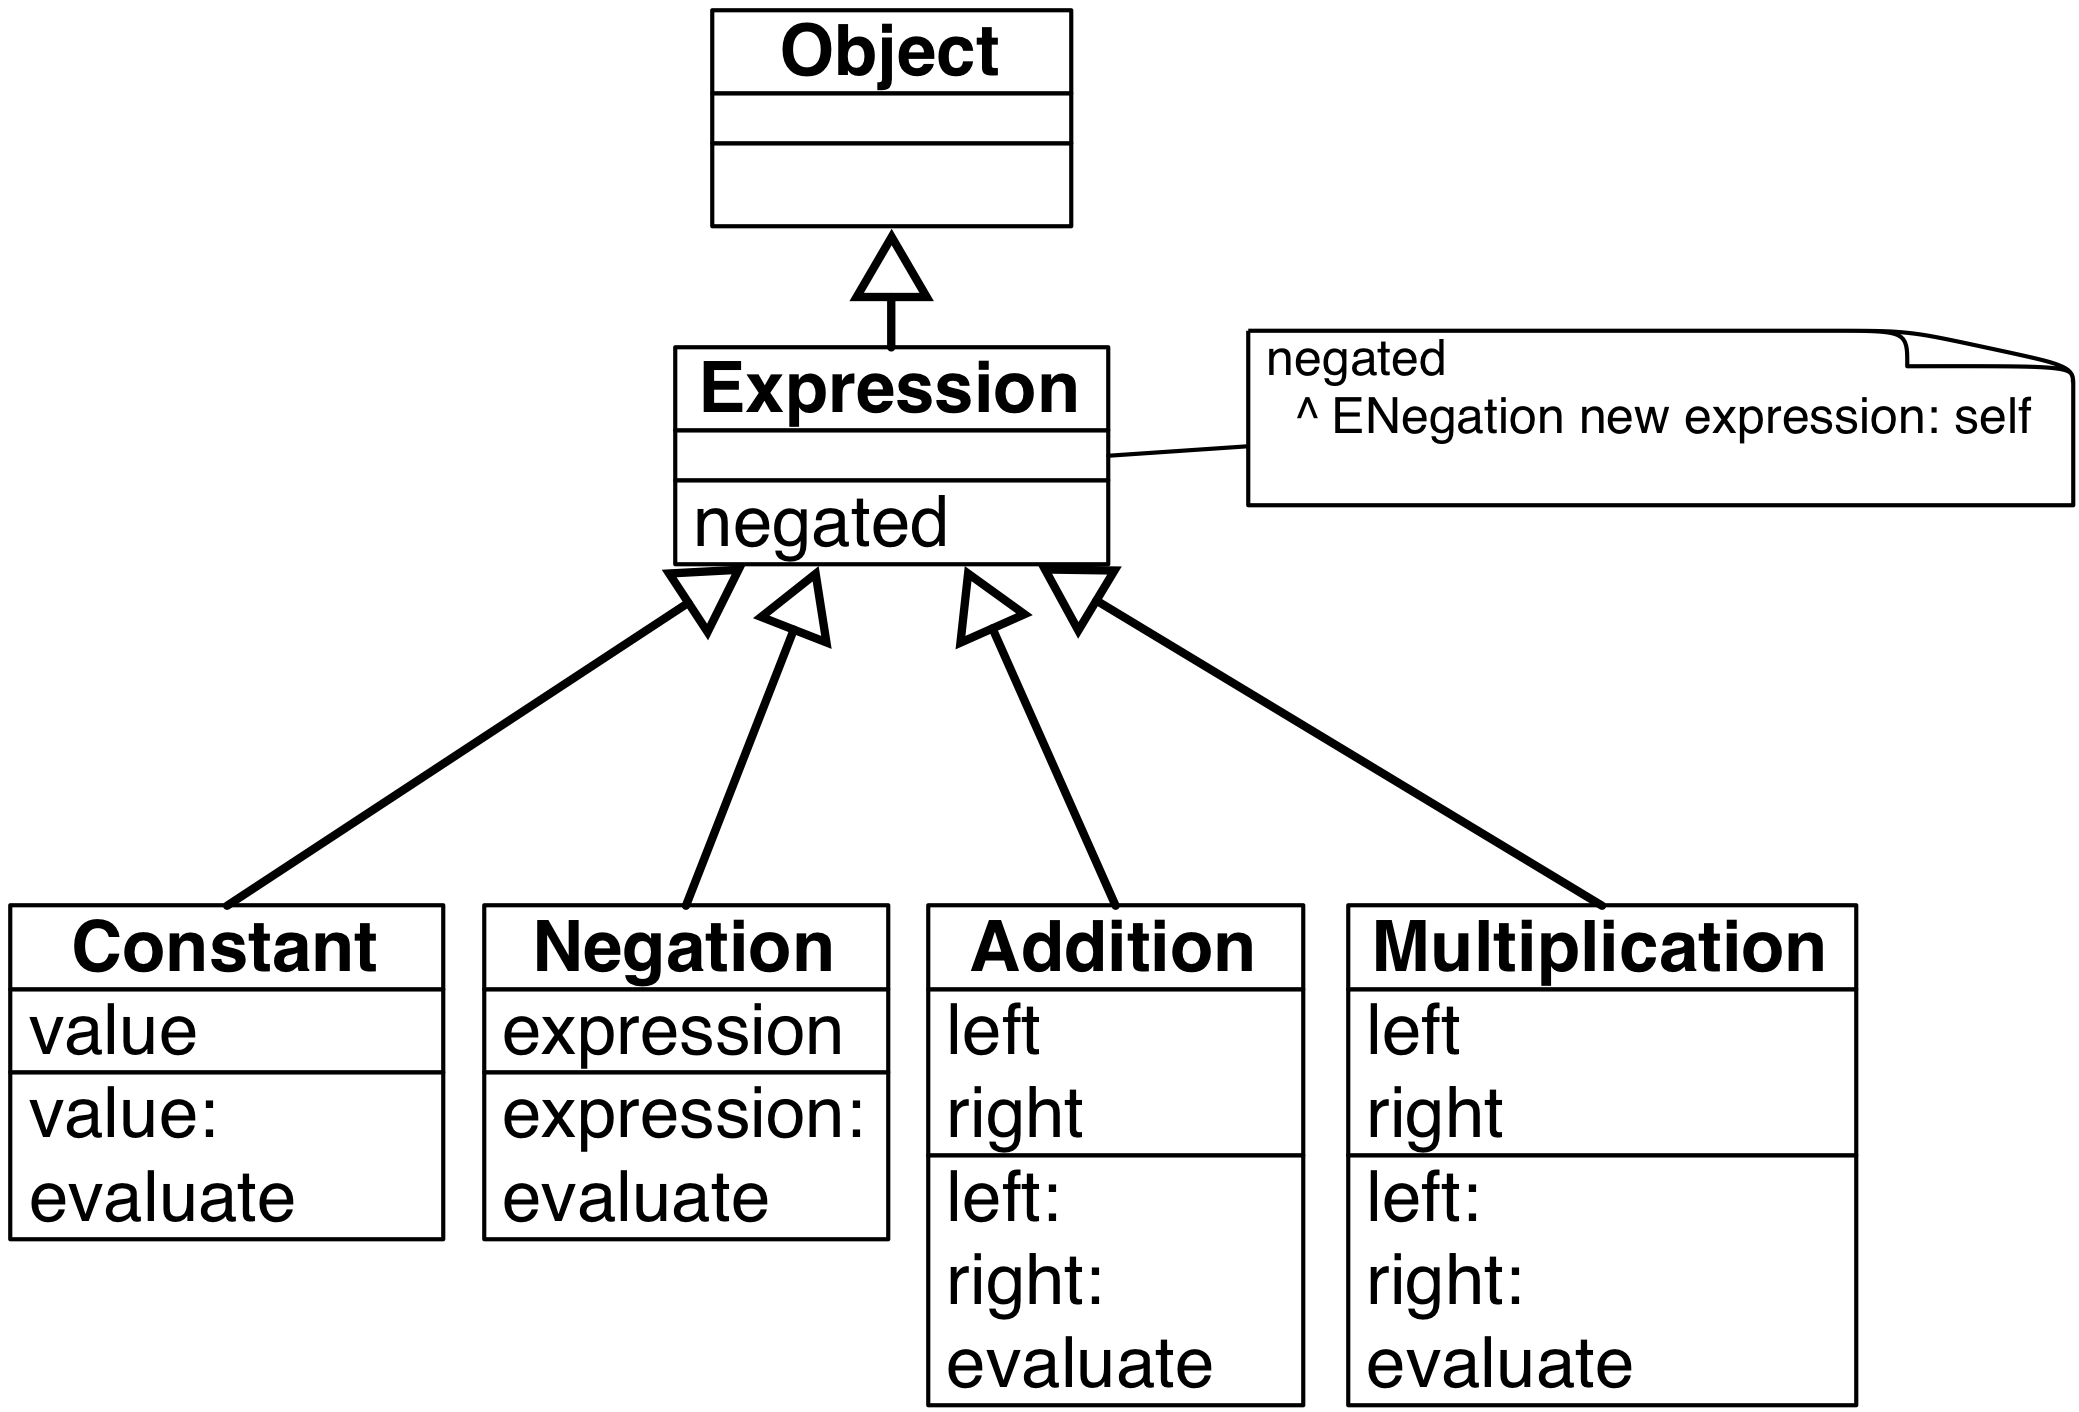
\includegraphics[width=0.7\textwidth]{/Users/ducasse/Workspace/FirstCircle/MyBooks/Bk-Writing/PharoBooks/LearningOOPWithPharoTrans/_result/pdf/Chapters/Expressions/figures/ExpressionsHierarchy.png}\caption{Introducing a common superclass.\label{figExpressionHierar}}\end{center}
\end{figure}


Let us introduce a new class to obtain the situation depicted by Figure \ref{figExpressionHierar}. 
We can simply do it by adding a new class:

\begin{displaycode}{plain}
Object subclass: #EExpression
	instanceVariableNames: ''
	classVariableNames: ''
	package: 'Expressions'
\end{displaycode}

and changing all the previous definitions to inherit from \textcode{EExpression} instead of \textcode{Object}.
For example the class \textcode{EConstant} is then defined as follows. 

\begin{displaycode}{plain}
EExpression subclass: #EConstant
	instanceVariableNames: 'value'
	classVariableNames: ''
	package: 'Expressions'
\end{displaycode}

We can also use for the first transformation the class refactoring \textit{Insert superclass}. Refactorings are code transformations that do not change the behavior of a program. You can find it under the refactorings list when you bring the menu on the classes. 
Now it is only useful for the first changes. 

Once the classes \textcode{EConstant}, \textcode{ENegation}, \textcode{EAddition}, and \textcode{EMultiplication} are subclasses of \textcode{EEXpression}, we should focus on the method \textcode{negated}. Now the method refactoring \textit{Push up} will really help us. 

\begin{itemize}
\item Select the method \textcode{negated} in one of the classes
\item Select the refactoring \textit{Push up}
\end{itemize}

The system will define the method \textcode{negated} in the superclass (\textcode{EExpression}) and remove all the negated methods in the classes. Now we obtain the situation described in Figure \ref{figExpressionHierar}. It is a good moment to run all your tests again. They should all pass. 

Now you could think that we can introduce a new class named ArithmeticExpression as a superclass of \textcode{EAddition} and \textcode{EMultiplication}. Indeed this is something that we could do to factor out common structure and behavior between the two classes. We will do it later because this is basically just a repetition of what we have done.
\section{Class creation messages}
Until now we always sent the message new to a class followed by a setter method as shown below. 

\begin{displaycode}{plain}
EConstant new value: 5
\end{displaycode}

We would like to take the opportunity to show that we can define simple \textbf{class} methods to improve the class instance creation interface. In this example it is simple and the benefits are not that important but we think that this is a nice example. With this in mind the previous example can now be written as follows: 

\begin{displaycode}{plain}
EConstant value: 5
\end{displaycode}

Notice the important difference that in the first case the message is sent to the newly created instance while in the second case it is sent to the class itself. 

To define a class method is the same as to define an instance method (as we did until now). The only difference is that using the code browser you should click on the classSide button to indicate that you are defining a method that should be executed in response
to a message sent to a class itself. 
\subsection{Better instance creation for constants}
Define the following method on the class \textcode{EConstant}. Notice the definition now use \textcode{EConstant class} and not just \textcode{EConstant} to stress that we are defining the class method. 

\begin{displaycode}{plain}
EConstant class >> value: anInteger
	^ self new value: anInteger
\end{displaycode}

Now define a new test to make sure that our method works correctly.

\begin{displaycode}{plain}
EConstantTest >> testCreationWithClassCreationMessage
	self assert: (EConstant value: 5) evaluate equals: 5
\end{displaycode}
\subsection{Better instance creation for  negations}
We do the same for the class \textcode{ENegation}.

\begin{displaycode}{plain}
ENegation class >> expression: anExpression
	... Your code ...
\end{displaycode}

We write of course a new test as follows: 

\begin{displaycode}{plain}
ENegationTest >> testEvaluateWithClassCreationMessage
	self assert: (ENegation expression: (EConstant value: 5)) evaluate equals: -5
\end{displaycode}
\subsection{Better instance creation for  additions}
For the addition we  add a class method named \textcode{left:right:} taking two arguments 

\begin{displaycode}{plain}
EAddition class >> left: anInteger right: anInteger2
	^ self new left: anInteger ; right: anInteger2 
\end{displaycode}

Of course, since we are addicted to tests, we add a new test. 

\begin{displaycode}{plain}
EEAdditionTest >> testEvaluateWithClassCreationMessage
	| ep1 ep2 |
	ep1 := EConstant constant5.
	ep2 := EConstant constant3.
	self assert: (EAddition left: ep1 right: ep2) evaluate equals: 8
\end{displaycode}
\subsection{Better instance creation for  multiplications}
We let you do the same for the multiplication. 

\begin{displaycode}{plain}
EMultiplication class >> left: anExp right: anExp2
	... Your code ...
\end{displaycode}

And another test to check that everything is ok. 

\begin{displaycode}{plain}
EMultiplicationTest >> testEvaluateWithClassCreationMessage
	| ep1 ep2 |
	ep1 := EConstant new value: 5.
	ep2 := EConstant new value: 3.
	self assert: (EMultiplication new left: ep1; right: ep2) evaluate equals: 15
\end{displaycode}

Run your tests! They should all pass. 
\section{Introducing examples as class messages}
As you saw when writing the tests, it is quite annoying to repeat all the time the expressions to get a given tree. This is especially the case in the tests related to addition and multiplication as the one below: 

\begin{displaycode}{plain}
EEAdditionTest >> testNegated
	| ep1 ep2 |
	ep1 := EConstant new value: 5.
	ep2 := EConstant new value: 3.
	self assert: (EAddition new right: ep1; left: ep2) negated evaluate equals: -8
\end{displaycode}

One simple solution is to define some class methods returning typical instances of their classes. To define a class method remember that you should click the class side button. 

\begin{displaycode}{plain}
EConstant class >> constant5
	^ self new value: 5
\end{displaycode}

\begin{displaycode}{plain}
EConstant class >> constant3
	^ self new value: 3
\end{displaycode}

This way we can define the test as follows:

\begin{displaycode}{plain}
EEAdditionTest >> testNegated
	| ep1 ep2 |
	ep1 := EConstant constant5.
	ep2 := EConstant constant3.
	self assert: (EAddition new right: ep1; left: ep2) negated evaluate equals: -8
\end{displaycode}

The tools in Pharo support such a practice. If we tag a class method with the special annotation \textcode{\textless{}sampleInstance\textgreater{}} the browser will show a little icon on the side and when we click on it, it will open an inspector on the new instance. 

\begin{displaycode}{plain}
EConstant class >> constant3
	<sampleInstance>
	^ self new value: 3
\end{displaycode}

using the same idea we defined the following class methods to return some examples of our classes.

\begin{displaycode}{plain}
EAddition class >> fivePlusThree
	<sampleInstance>
	| ep1 ep2 |
	ep1 := EConstant new value: 5.
	ep2 := EConstant new value: 3.
	^ self new left: ep1 ; right: ep2 
\end{displaycode}

\begin{displaycode}{plain}
EMultiplication class >> fiveTimesThree
	<sampleInstance>
	| ep1 ep2 |
	ep1 := EConstant constant5.
	ep2 := EConstant constant3.
   ^ EMultiplication new left: ep1 ; right: ep2 
\end{displaycode}

What is nice with such examples is that 

\begin{itemize}
\item they help documenting the class by providing objects that we can directly use,
\item they support the creation of tests by providing objects that can serve as input for tests,
\item they simplify the writing of tests. 
\end{itemize}

So think to use them. 
\section{Printing}
It is quite annoying that we cannot really see an expression when we inspect it. We would like to get something better than \textcode{'aEConstant'} and \textcode{'anEAddition'} when we debug our programs.
To display such information the debugger and inspector send to the objects the message \textcode{printString} which by default just prefix the name of the class with 'an' or 'a'. 

Let us change this situation. For this, we will specialize the method \textcode{printOn: aStream}. The message \textcode{printOn:} is called on the object when a program or the system send to the object the message \textcode{printString}. From that perspective \textcode{printOn:} is a system customization point that developers can take advantage to enhance their programming experience.

Note that we do not redefine the method \textcode{printString} because it is more complex and \textcode{printString} is reused for all the objects in the system. We just have to implement the part that is specific to a given class. In object-oriented design jargon, \textcode{printString} is a template method in the sense that it sets up a context which is shared by other objects and it hosts hook methods which are program customization points. \textcode{printOn:} is a hook method. The term hook comes from the fact that code of subclasses are invoked in the hook place (see Figure \ref{fig:ExpressionsHierarchyPrintOn}).

The default definition of the method \textcode{printOn:} as defined on the class \textcode{Object} is the following: it grabs the class name and checks if it starts with a vowel or not and write to the stream the 'a/an class'. This is why by default we got \textcode{'anEConstant'} when we printed a constant expression. 

\begin{displaycode}{plain}
Object >> printOn: aStream
	"Append to the argument, aStream, a sequence of characters that  
	identifies the receiver."
	| title |
	title := self class name.
	aStream
		nextPutAll: (title first isVowel ifTrue: ['an '] ifFalse: ['a ']);
		nextPutAll: title
\end{displaycode}


\begin{figure}

\begin{center}
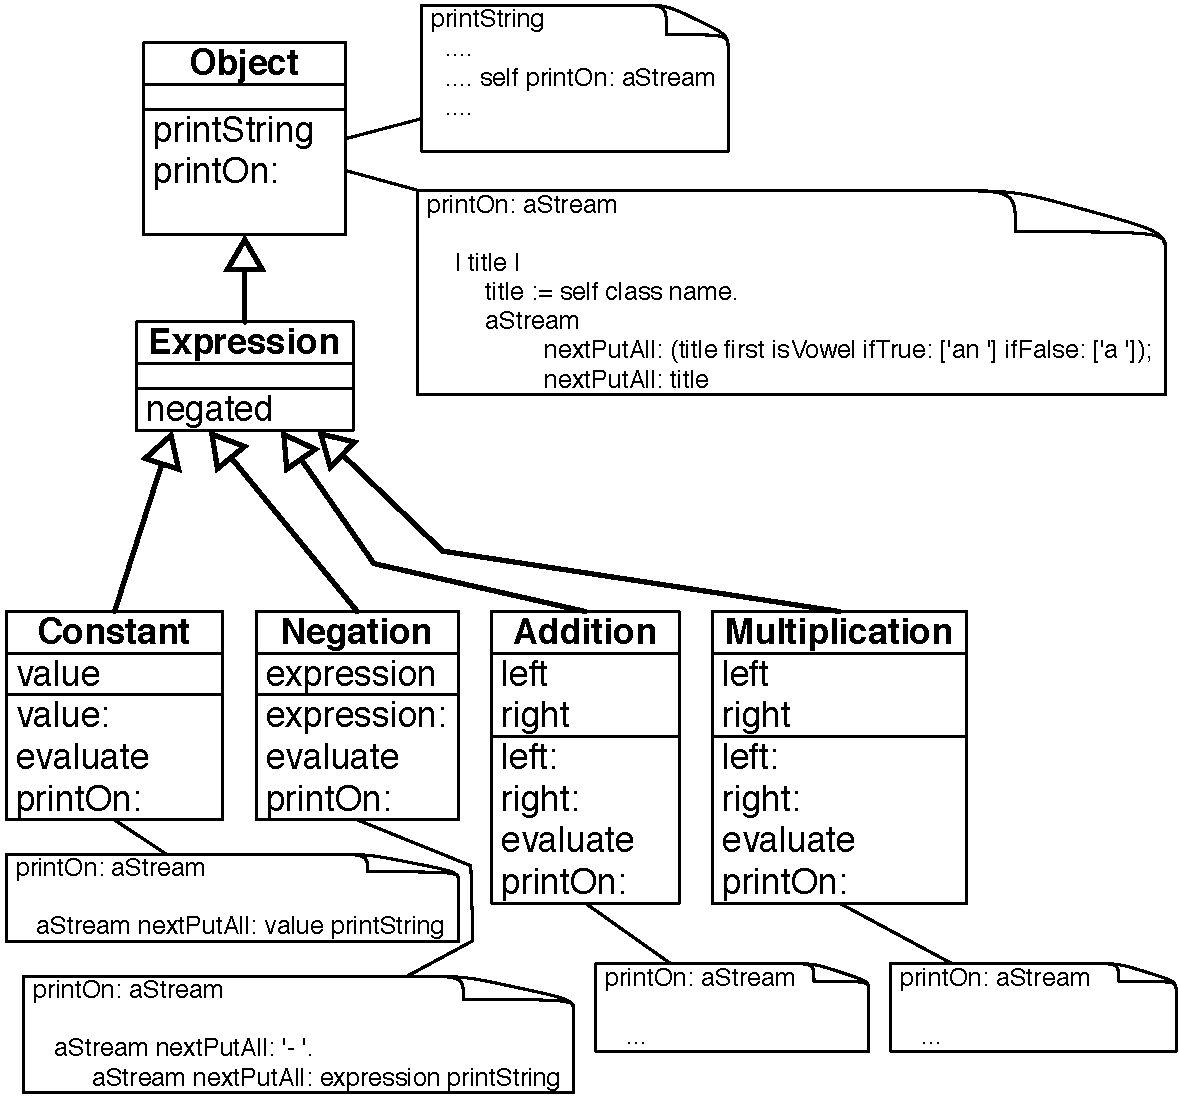
\includegraphics[width=0.7\textwidth]{/Users/ducasse/Workspace/FirstCircle/MyBooks/Bk-Writing/PharoBooks/LearningOOPWithPharoTrans/_result/pdf/Chapters/Expressions/figures/ExpressionsHierarchyPrintOn.pdf}\caption{printOn: and printString a \symbol{34}hooks and template\symbol{34} in action.\label{fig:ExpressionsHierarchyPrintOn}}\end{center}
\end{figure}

\subsection{A word about streams}
A stream is basically a container for a sequence of objects. Once we get a stream we can either read from it or write to it. In our case we will write to the stream. Since the stream passed to printOn: is a stream expecting characters we will add characters or strings (sequence of characters) to it. We will use the messages: \textcode{nextPut: aCharacter} and \textcode{nextPutAll: aString}. 
They add to the stream the arguments at the next position and following. We will guide you and it is simple. 
You can find more information on the chapter about Stream in the book: Pharo by Example available at \url{http://books.pharo.org}
\subsection{Printing constant}
Let us start with a test. Here we check that a constant is printed as its value.

\begin{displaycode}{plain}
EConstantTest >> testPrinting
	self assert: (EConstant value: 5) printString equals: '5'
\end{displaycode}

The implementation is then simple. We just need to put the value converted as a string to the stream.
 

\begin{displaycode}{plain}
EConstant >> printOn: aStream
	aStream nextPutAll: value printString
\end{displaycode}
\subsection{Printing negation}
For a negation we should first put a '-' and then recurvisely call the printing process on the negated expression. Remember that sending the message \textcode{printString} to an expression should return its string representation.  At least until now it will work for constants. 

\begin{displaycode}{plain}
(EConstant value: 6) printString
>>> '6'
\end{displaycode}

Here is a possible definition

\begin{displaycode}{plain}
ENegation >> printOn: aStream
	aStream nextPutAll: '- '
	aStream nextPutAll: expression printString
\end{displaycode}

By the way since all the messages are sent to the same object, this method can be rewritten as:

\begin{displaycode}{plain}
ENegation >> printOn: aStream
	aStream 
		nextPutAll: '- ';
		nextPutAll: expression printString
\end{displaycode}

We can also define it as follows: 

\begin{displaycode}{plain}
ENegation >> printOn: aStream
	aStream nextPutAll: '- '.
	expression printOn: aStream
\end{displaycode}

The difference between the first solution and the alternate implementation is the following:
In the solution using \textcode{printString}, the system creates two streams: one for each invocation of the message \textcode{printString}. One for printing the expression and one for printing the negation. Once the first stream is used the message \textcode{printString} converts the stream contents into a string and this new string is put inside the second stream which at the end is converted again as a string. So the first solution is not really efficient. 
With the second solution, only one stream is created and each of the method just put the needed string elements inside. 
At the end of the process, the single \textcode{printString} message converts it into a string. 
\subsection{Printing addition}
Now let us write yet another test for addition printing. 

\begin{displaycode}{plain}
EAdditionTest >> testPrinting
	self assert: (EAddition fivePlusThree) printString equals:  '( 5 + 3 )'.
	self assert: (EAddition fivePlusThree) negated printString equals:  '- ( 5 + 3 )'
\end{displaycode}

Printing an addition is: put an open parenthesis, print the left expression, put ' + ', print the right expression and put a closing parenthesis in the stream. 

\begin{displaycode}{plain}
EAddition >> printOn: aStream
	... Your code ...
\end{displaycode}
\subsection{Printing multiplication}
And now we do the same for multiplication. 

\begin{displaycode}{plain}
EMultiplicationTest >> testPrinting
	self assert: (EMultiplication fiveTimesThree) negated printString equals:  '- ( 5 * 3 )'
\end{displaycode}

\begin{displaycode}{plain}
EMultiplication >> printOn: aStream
	... Your code ...
\end{displaycode}
\section{Revisiting negated message for Negation}
Now we can go back on negating an expression. Our implementation is not nice even if we can negate any expression and get the correct value. If you look at it carefully negating a negation could be better. 
Printing a negated negation illustrates well the problem: we get two minuses instead of none. 

\begin{displaycode}{plain}
(EConstant value: 11) negated 
>> '- 11'

(EConstant value: 11) negated negated
>> '- - 11'
\end{displaycode}

A solution could be to change the printOn: definition and to check if the expression that is negated is a negation 
and in such case to not emit the minus. Let us say it now, this solution is not nice because we do not want to write code
that depends on explicitly checking if an object is of a given class. Remember we want to send message and let the object do some actions. 

A good solution is to \textit{specialize} the message \textcode{negated} so that when it is sent to a \textit{negation} it does not create a new negation that points to the receiver but instead returns the expression itself, otherwise the method implemented in \textcode{EExpression} will be executed. This way the trees created by a \textcode{negated} message can never have negated negation but the arithmetic values obtained are correct. Let us implement this solution, we just need to implement a different version of the method \textcode{negated} for \textcode{ENegation}. 

Let us write a test! Since evaluating a single expression or a double negated one gives the same results, we need to define a structural test. This is what we do with the expression \textcode{exp negated class = ENegation} below.

\begin{displaycode}{plain}
NegationTest >> testNegatedStructureIsCorrect
	| exp |
	exp := EConstant value: 11.
	self assert: exp negated class = ENegation. 
	self assert: exp negated negated equals: exp.
\end{displaycode}

Now you should be able to implement the \textcode{negated} message on \textcode{ENegation}. 

\begin{displaycode}{plain}
ENegation >> negated
	... Your code ...
\end{displaycode}
\subsection{Understanding method override}
When we send a message to an object, the system looks for the corresponding method in the class of the receiver then if it is not defined there, the lookup continues in the superclass of the previous class. 

By adding a method in the class \textcode{ENegation}, we created the situation shown in Figure \ref{fig:ExpressionsHierarchyOptimized}. We said that the message \textcode{negated} is overridden in \textcode{ENegation} because for instances of \textcode{ENegation} it hides the method defined in the superclass \textcode{EExpression}. 

It works the following:

\begin{itemize}
\item When we send the message \textcode{negated} to a constant, the message is not found in the class \textcode{EConstant} and then it is looked up in the class \textcode{EExpression} and it is found there and applied to the receiver (the instance of \textcode{EConstant}).
\end{itemize}

\begin{itemize}
\item When we send the message \textcode{negated} to a negation, the message is found in the class \textcode{ENegation} and executed on the negation expression. 
\end{itemize}


\begin{figure}

\begin{center}
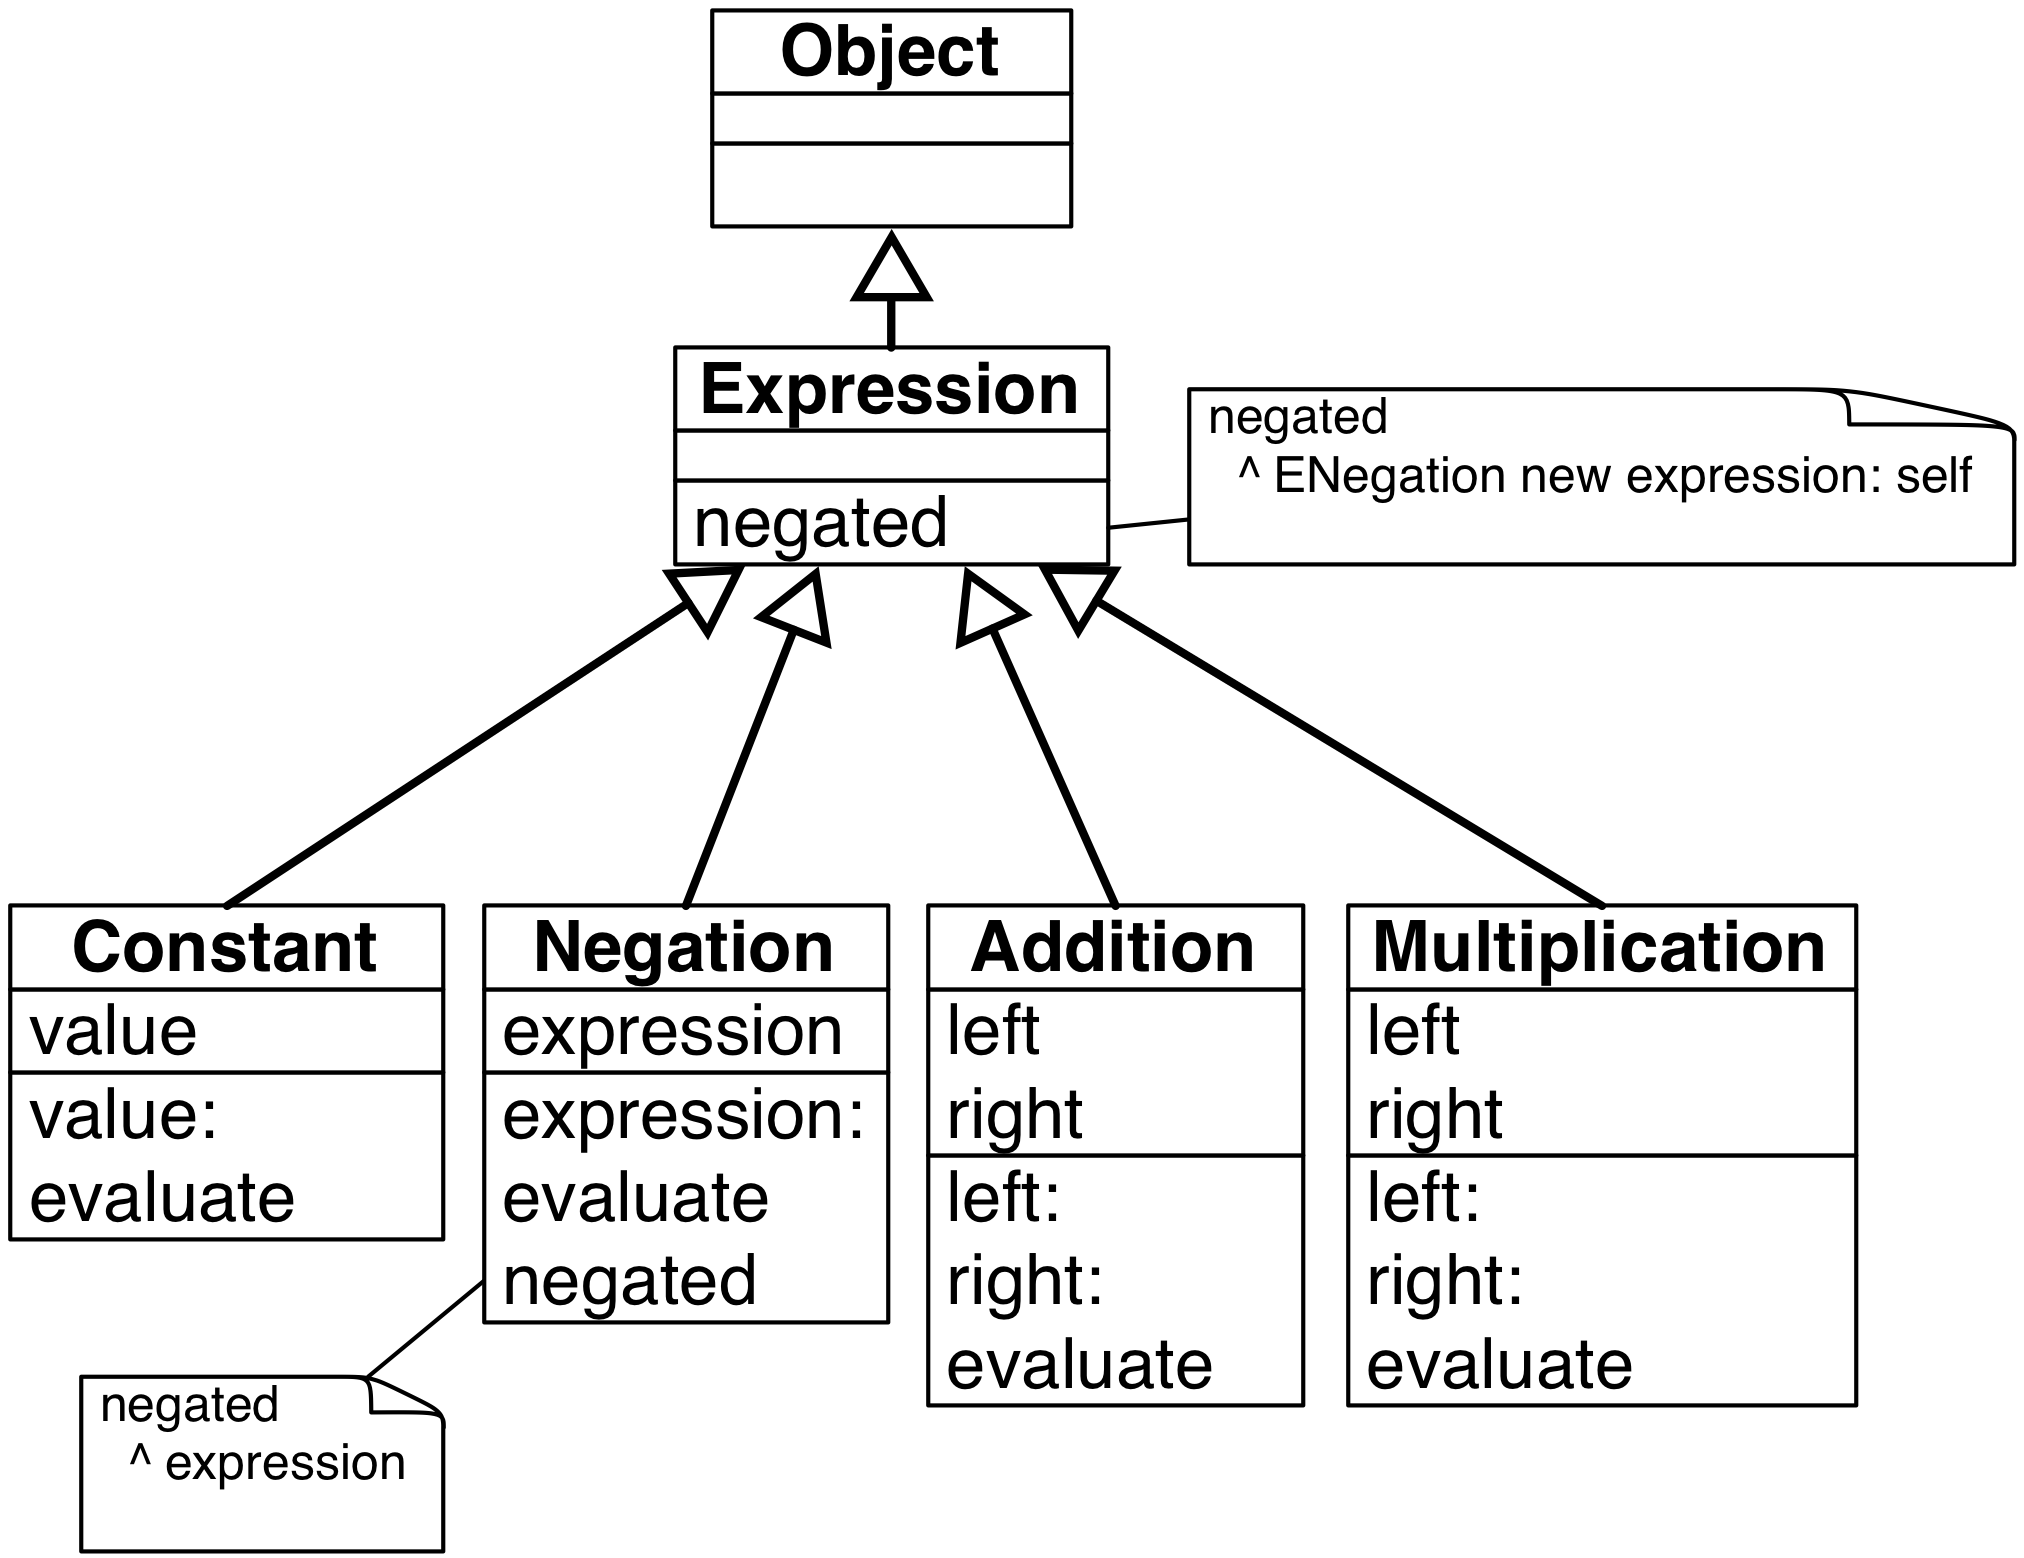
\includegraphics[width=0.7\textwidth]{/Users/ducasse/Workspace/FirstCircle/MyBooks/Bk-Writing/PharoBooks/LearningOOPWithPharoTrans/_result/pdf/Chapters/Expressions/figures/ExpressionsHierarchyOptimized.png}\caption{The message \textcode{negated} is overridden in the class \textcode{ENegation}.\label{fig:ExpressionsHierarchyOptimized}}\end{center}
\end{figure}

\section{Introducing BinaryExpression class}\label{secBinaryExpression}
Now we will take a moment to improve our first design. We will factor out the behavior of \textcode{EAddition} and \textcode{EMultiplication}. 

\begin{displaycode}{plain}
EExpression subclass: #EBinaryExpression
	instanceVariableNames: ''
	classVariableNames: ''
	package: 'Expressions'
\end{displaycode}

\begin{displaycode}{plain}
EBinaryExpression subclass: #EAddition
	instanceVariableNames: 'left right'
	classVariableNames: ''
	package: 'Expressions'
\end{displaycode}

\begin{displaycode}{plain}
EBinaryExpression subclass: #EMultiplication
	instanceVariableNames: 'left right'
	classVariableNames: ''
	package: 'Expressions'
\end{displaycode}

Now we can use again a refactoring to pull up the instance variables \textcode{left} and \textcode{right}, as well as the methods \textcode{left:} and \textcode{right:}.

Select the class \textcode{EMuplication}, bring the menu and select in the Refactoring menu the instance variables refactoring \textit{Push Up}. Then select the instance variables.

Now you should get the following class definitions, where the instance variables are defined in the new class and removed from the two subclasses. 

\begin{displaycode}{plain}
EExpression subclass: #EBinaryExpression
	instanceVariableNames: 'left right'
	classVariableNames: ''
	package: 'Expressions'
\end{displaycode}

\begin{displaycode}{plain}
EBinaryExpression subclass: #EAddition
	instanceVariableNames: ''
	classVariableNames: ''
	package: 'Expressions'
\end{displaycode}

\begin{displaycode}{plain}
EBinaryExpression subclass: #EMultiplication
	instanceVariableNames: ''
	classVariableNames: ''
	package: 'Expressions'
\end{displaycode}

We should get a situation similar to the one of Figure \ref{figExpressionFactoredState}. All your tests should still pass. 


\begin{figure}

\begin{center}
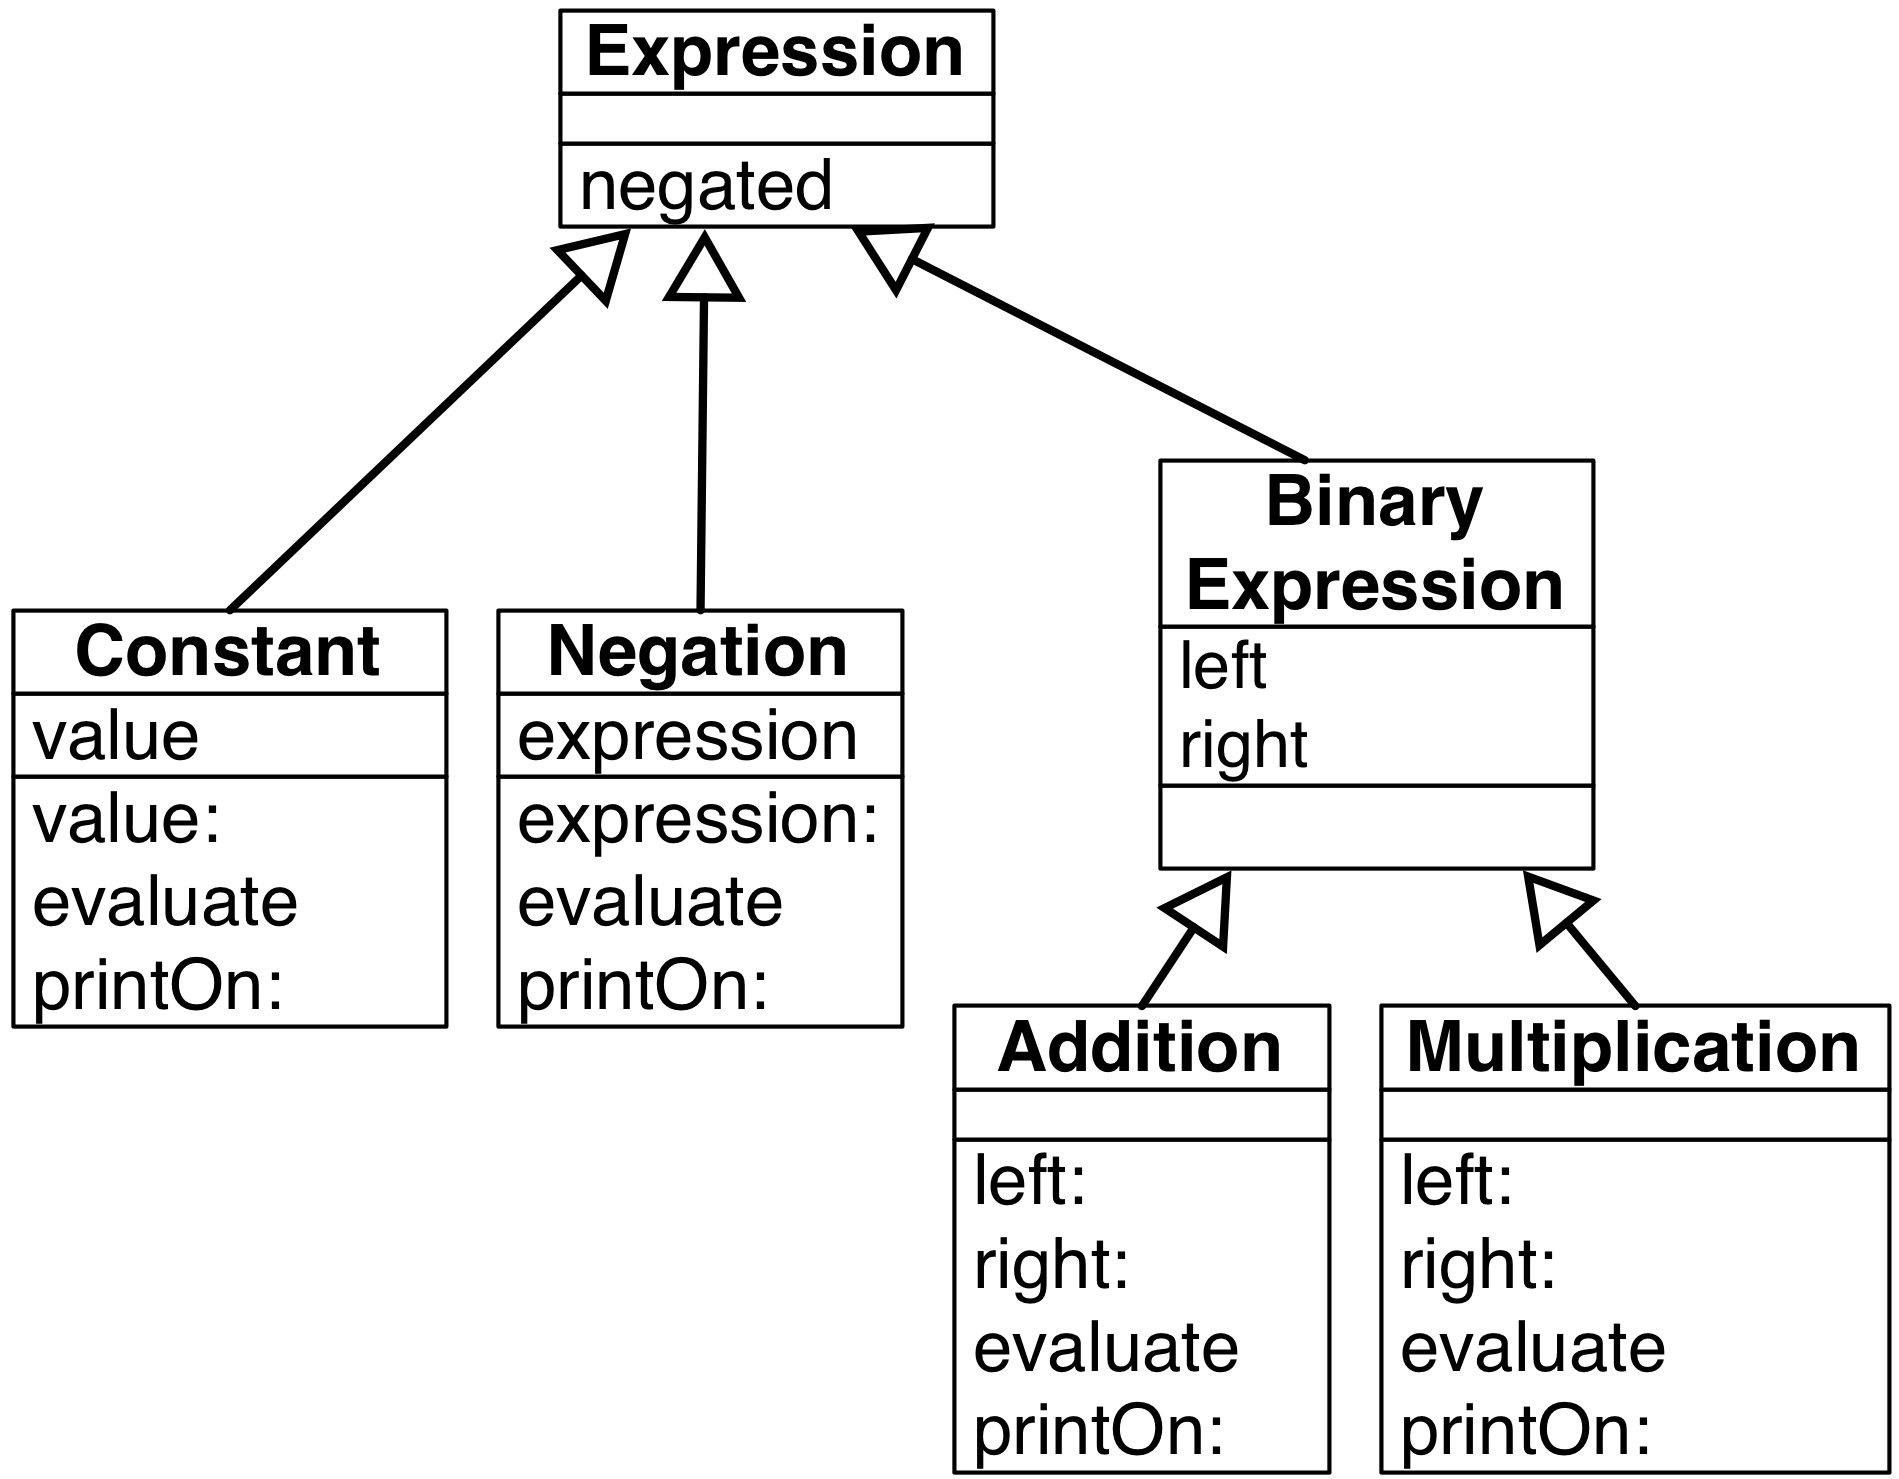
\includegraphics[width=0.7\textwidth]{/Users/ducasse/Workspace/FirstCircle/MyBooks/Bk-Writing/PharoBooks/LearningOOPWithPharoTrans/_result/pdf/Chapters/Expressions/figures/ExpressionsHierarchyStateFactored.png}\caption{Factoring instance variables.\label{figExpressionFactoredState}}\end{center}
\end{figure}


Now we can move the same way the methods. Select the method \textcode{left:} and apply the refactoring \textit{Pull Up Method}.  Do the same for the method \textcode{right:}. 
\subsection{Creating a template and hook method}
Now we can look at the methods \textcode{printOn:} of additions and multiplications. They are really similar: Just the operator is changing. Now we cannot simply copy one of the definitions because it will not work for the other. But what we can do is to apply the same design point that implemented for \textcode{printString} and \textcode{printOn:}: we can create a template and hooks that will be specialized in the subclasses. 

We will use the method \textcode{printOn:} as a template with a hook redefined in each subclass.

Let define the method \textcode{printOn:} in \textcode{EBinaryExpression} and remove the other ones from the two classes \textcode{EAddition} and \textcode{EMultiplication}. 

\begin{displaycode}{plain}
EBinaryExpression >> printOn: aStream
	aStream nextPutAll: '( '.
	left printOn: aStream. 
	aStream nextPutAll: ' + '.
	right printOn: aStream.
	aStream nextPutAll: ' )'
\end{displaycode}

Then you can do it manually or use the \textit{Extract Method} Refactoring: This refactoring creates a new method from a part of an existing method and sends a message to the new created method: select the ' + ' inside the method pane and bring the menu and select the Extract Method refactoring, and when prompt give the name \textcode{operatorString}. 

Here is the result you should get:  

\begin{displaycode}{plain}
EBinaryExpression >> printOn: aStream
	aStream nextPutAll: '( '.
	left printOn: aStream.
	aStream nextPutAll: self operatorString.
	right printOn: aStream.
	aStream nextPutAll: ' )'
\end{displaycode}

\begin{displaycode}{plain}
EBinaryExpression >> operatorString
	^ ' + '
\end{displaycode}

Now we can just redefine this method in the \textcode{EMultiplication} class to return the adequate string.

\begin{displaycode}{plain}
EMultiplication >> operatorString
	^ ' * '
\end{displaycode}


\begin{figure}

\begin{center}
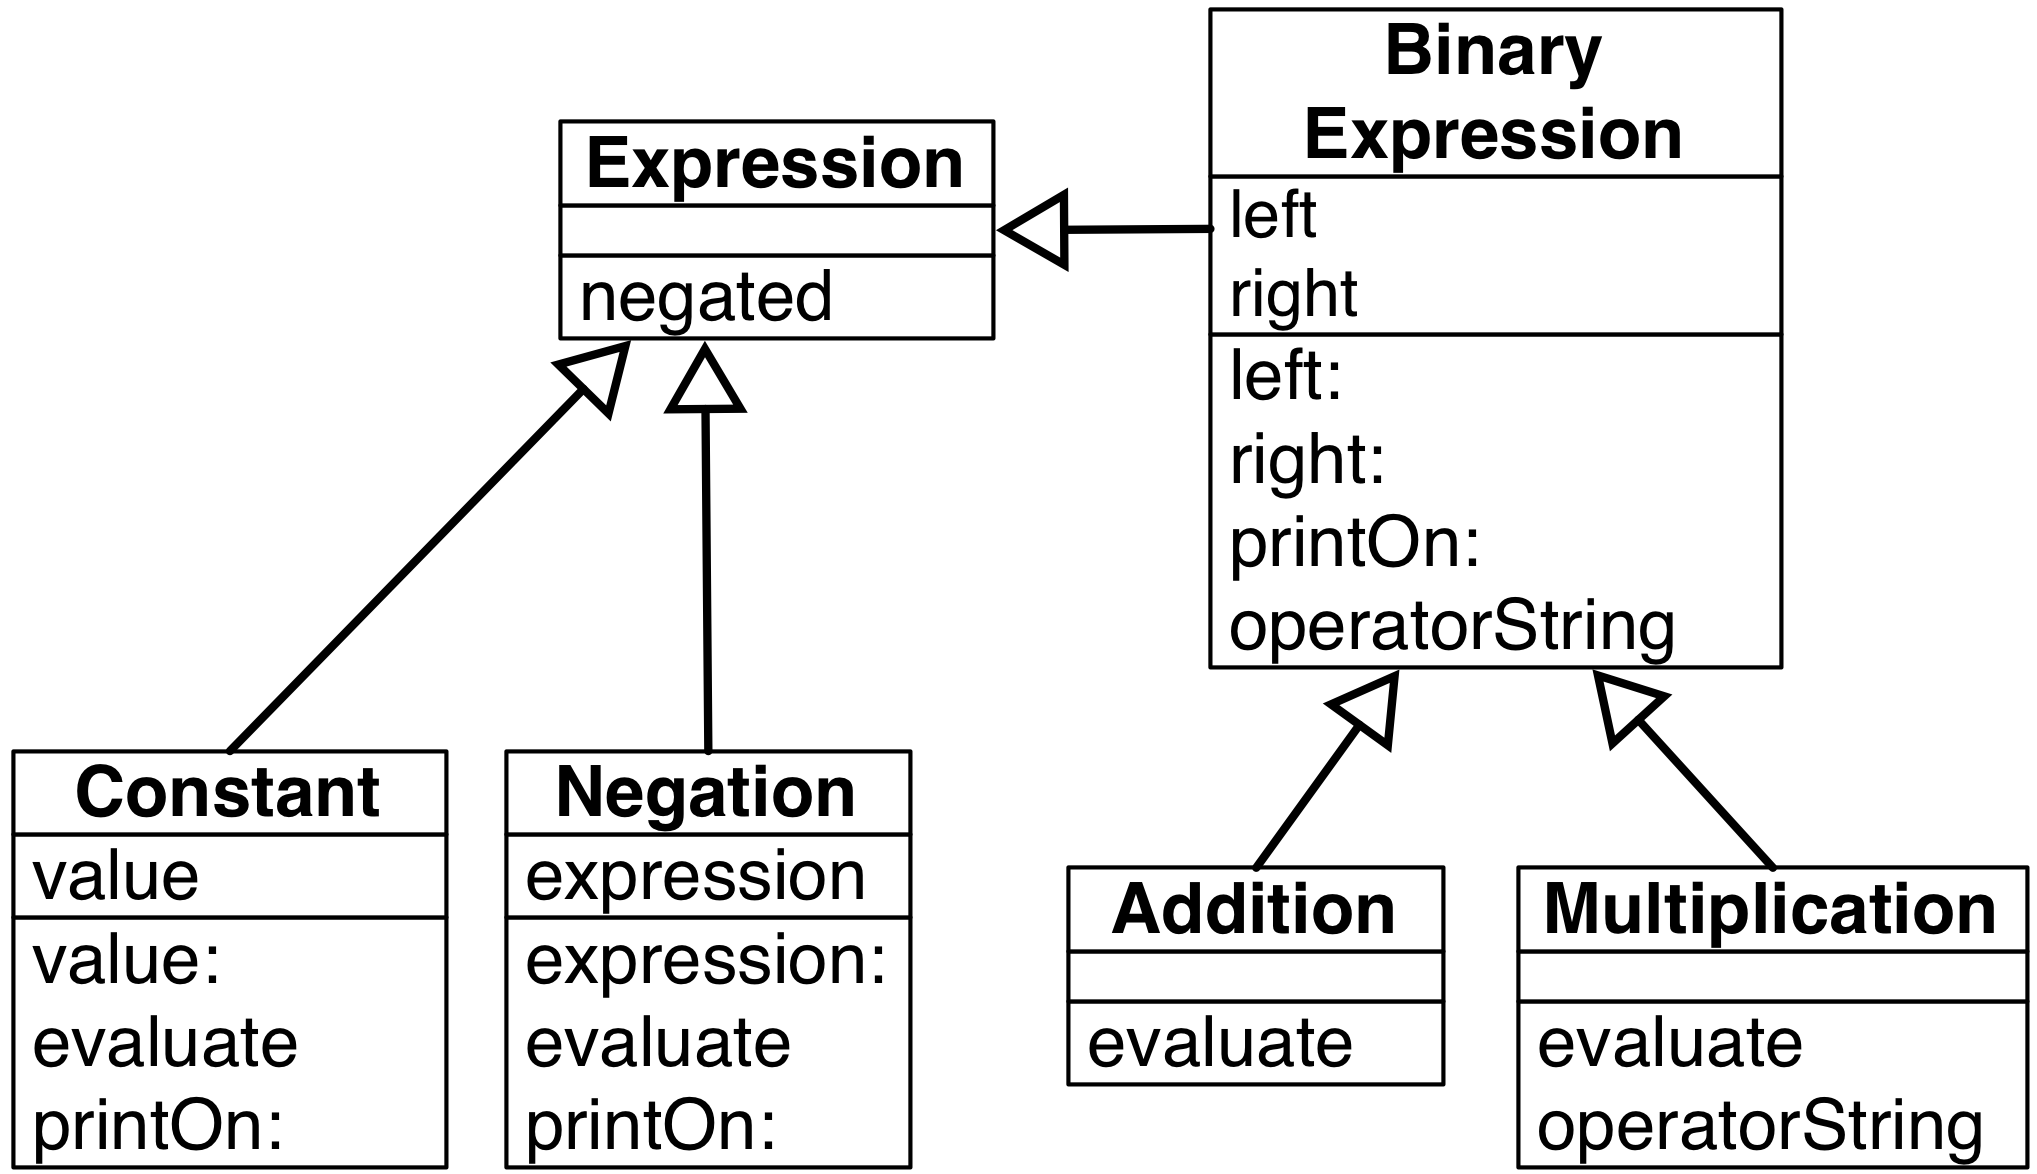
\includegraphics[width=0.7\textwidth]{/Users/ducasse/Workspace/FirstCircle/MyBooks/Bk-Writing/PharoBooks/LearningOOPWithPharoTrans/_result/pdf/Chapters/Expressions/figures/ExpressionsHierarchyStateBehaviorFactored.png}\caption{Factoring instance variables and behavior.\label{figExpressionsHierarchyStateBehaviorFactored}}\end{center}
\end{figure}

\section{What did we learn}
The introduction of the class \textcode{EBinaryExpression} is a rich experience in terms of lessons that we can learn. 

\begin{itemize}
\item Refactorings are more than simple code transformations. Usually refactorings pay attention that their application does not change the behavior of programs. As we saw refactorings are powerful operations that really help doing complex operations in a few action.
\end{itemize}

\begin{itemize}
\item We saw that the introduction of a new superclass and moving instance variables or method to a superclass does not change the structure or behavior of the subclasses. This is because (1) for the state, the structure of an instance is based on the state of its class and all its superclasses, (2) the lookup starts in the class of the receiver and look in superclasses.
\end{itemize}

\begin{itemize}
\item While the method \textcode{printOn:} is by itself a hook for the method \textcode{printString}, it can also play the role of a template method. The method \textcode{operatorString} reuses the context created by the \textcode{printOn:} method which acts as a template method. In fact each time we do a self send we create a hook method that subclasses can specialize.
\end{itemize}
\section{About hook methods}
When we introduced \textcode{EBinaryExpression} we defined the method \textcode{operatorString} as follows:

\begin{displaycode}{plain}
EBinaryExpression >> operatorString
	^ ' + '
\end{displaycode}

\begin{displaycode}{plain}
EMultiplication >> operatorString
	^ ' * '
\end{displaycode}

And you may wonder if it was worth to create a new method in the superclass and so that such one subclass redefines it. 
\subsection{Creating hooks is always good}
First creating a hook is also a good idea. Because you rarely know how your system will be extended in the future. On this little example, we suggest you to add raising to power, division and this can be done with one class and two methods per new operator. 
\subsection{Avoid not documenting hooks}
Second we could have just defined one method \textcode{operatorString} in each subclass and no method in the superclass \textcode{EBinaryExpression}. It would have worked because \textcode{EBinaryExpression} is not meant to have direct instances. Therefore there is no risk that a \textcode{printOn:} message is sent to one of its instance and cause an error because no method \textcode{operatorString} is found. 

The code would have looked like the following: 

\begin{displaycode}{plain}
EAddition >> operatorString
	^ ' + '
\end{displaycode}

\begin{displaycode}{plain}
EMultiplication >> operatorString
	^ ' * '
\end{displaycode}


\begin{figure}

\begin{center}
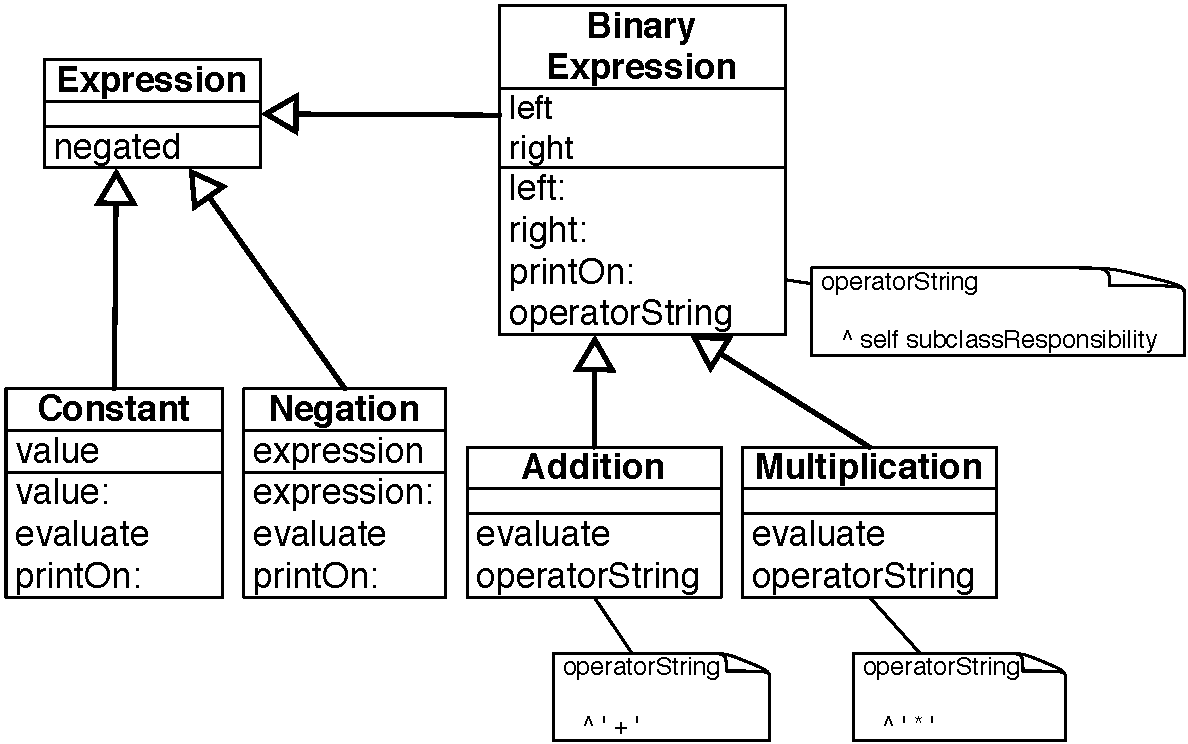
\includegraphics[width=0.7\textwidth]{/Users/ducasse/Workspace/FirstCircle/MyBooks/Bk-Writing/PharoBooks/LearningOOPWithPharoTrans/_result/pdf/Chapters/Expressions/figures/ExpressionsHierarchyBinaryAbstract.pdf}\caption{Better design: Declaring an abstract method as a way to document a hook method.\label{figExpressionsHierarchyBinaryAbstract}}\end{center}
\end{figure}


Now such a design is not really good because as potential extenders, developers will have to guess reading the subclass definitions that they should also define a method \textcode{operatorString}. A better solution in that case is to define an \textit{abstract} method in the superclass as follows: 

\begin{displaycode}{plain}
EBinaryExpression >> operatorString
	^ self subclassResponsibility
\end{displaycode}

Using the message \textcode{subclassResponsibility} declares that a method is abstract and does nothing except forcing its redefinition: subclasses should redefine it explicitly. Using such an approach we get the final situation represented in Figure \ref{figExpressionsHierarchyBinaryAbstract}. 

In the solution presented before (section \ref{secBinaryExpression}) we decided to go for the simplest solution and it was to use one of the default value (' + ') as a default definition for the hook in the superclass \textcode{EExpression}.  It was not a good solution and we did it on purpose to be able to have this discussion. It was not a good solution since it was using a specific subclass. It is better to define a default value for a hook in the superclass when this default value makes sense in the class itself.

Note that we could also define \textcode{evaluate} as an abstract method in \textcode{EExpression} to indicate clearly that each subclass should 
define an \textcode{evaluate}.
\section{Variables}
Up until now our mathematical expressions are rather limited. We only manipulate constant-based expressions. What we would like is to be able to manipulate variables too. 
Here is a simple test to show what we mean: we define a variable named \textcode{'x'} and then we can later specify that \textcode{'x'} should take a given value. 

Let us create a new test class named \textcode{EVariableTest} and define a first test \textcode{testValueOfx}.

\begin{displaycode}{plain}
EVariableTest >> testValueOfx
	self assert: ((EVariable new id: #x) evaluateWith: {#x -> 10} asDictionary) equals: 10.
\end{displaycode}
\subsection{Some technical points}
Let us explain a bit what we are doing with the expression \textcode{\{\#x -\textgreater{} 10\} asDictionary}. We should be able to specify that a given variable name is associated with a given value. For this we create a dictionary: a dictionary is a data structure for storing keys and their associated value. Here a key is the variable and the value its associated value. Let us present some details first.
\subsubsection{Dictionaries}
A dictionary is a data structure containing pairs (key value) and we can access the value of a given key. It can use any object as key and any object as values. Here we simply use a symbol \textcode{\#x} since symbols are unique within the system and as such we are sure that we cannot have two keys looking the same but having different values. 

\begin{displaycode}{plain}
| d |
d := Dictionary new
	at: #x put: 33;
	at: #y put: 52;
	at: #z put: 98.
d at: y
>>> 52 
\end{displaycode}

The previous dictionary can be easily expressed more compactly using \textcode{\{\#x -\textgreater{} 33 . \#y -\textgreater{} 52 . \#z -\textgreater{} 98\} asDictionary}.

\begin{displaycode}{plain}
{#x -> 33 . #y -> 52 . #z -> 98} asDictionary at: #y
>>> 52 
\end{displaycode}
\subsubsection{Dynamic Arrays}
The expression \textcode{\{ \}} creates a dynamic array. Dynamic arrays execute their expressions and store the resulting values. 

\begin{displaycode}{plain}
{2 + 3 . 6 - 2 . 7-2 }
>>> #(5 4 5)
\end{displaycode}
\subsubsection{Pairs}
The expression \textcode{\#x -\textgreater{} 10} creates a pair with a key and a value.

\begin{displaycode}{plain}
| p |
p := #x -> 10.
p key 
>>> #x
p value
>>> 10
\end{displaycode}
\subsection{Back to variable expressions}
If we go a step further, we want to be able to build more complex expressions where instead of having constants we can manipulate variables. This way we will be able to build more advanced behavior such as expression derivations. 

\begin{displaycode}{plain}
EExpression subclass: #EVariable
	instanceVariableNames: 'id'
	classVariableNames: ''
	package: 'Expressions'
\end{displaycode}

\begin{displaycode}{plain}
EVariable >> id: aSymbol
	id := aSymbol
\end{displaycode}

\begin{displaycode}{plain}
EVariable >> printOn: aStream
	aStream nexPutAll: id asString
\end{displaycode}

What we see is that we need to be able to pass bindings (a binding is a pair key, value) when evaluating a variable. The value of a variable is the value of the binding whose key is the name of the variable. 

\begin{displaycode}{plain}
EVariable >> evaluateWith: aBindingDictionary
	^ aBindingDictionary at: id
\end{displaycode}

Your tests should all pass at this point. 

For more complex expressions (the ones that interest us) here are two tests. 

\begin{displaycode}{plain}
EVariableTest >> testValueOfxInNegation
	self assert: ((EVariable new id: #x) negated
		evaluateWith: {#x -> 10} asDictionary) equals: -10
\end{displaycode}

What the second test shows is that we can have an expression and given a different set of bindings the value of the expression will differ. 

\begin{displaycode}{plain}
EVariableTest >> testEvaluateXplusY
	| ep1 ep2 add |
	ep1 := EVariable new id: #x.
	ep2 := EVariable new id: #y.
	add := EAddition left: ep1 right: ep2.
	
	self assert: (add evaluateWith: { #x -> 10 . #y -> 2 } asDictionary) equals: 12.
	self assert: (add evaluateWith: { #x -> 10 . #y -> 12 } asDictionary) equals: 22
\end{displaycode}
\subsection{Non working approaches}
A non working solution would be to add the following method to \textcode{EExpression}

\begin{displaycode}{plain}
EEXpression >> evaluateWith: aDictionary
	^ self evaluate
\end{displaycode}

However it does not work for at least the following reasons: 

\begin{itemize}
\item It does not use its argument. It only works for trees composed out exclusively of constant. 
\item When we send a message \textcode{evaluateWith:} to an addition, this message is then turned into an \textcode{evaluate} message sent to its subexpression and such subexpression do not get an \textcode{evaluateWith:} message but an \textcode{evaluate}.
\end{itemize}

Alternatively we could add the binding to the variable itself and only provide an \textcode{evaluate} message as follows: 

\begin{displaycode}{plain}
(EVariable new id: #x) bindings: { #x -> 10 . #y -> 2 } asDictionary
\end{displaycode}

 But it fully defeats the purpose of what a variable is. We should be able to give different values to a variable embedded inside a complex expression.
\subsection{The solution: adding evaluateWith:}
We should transform all the implementations and message sends from \textcode{evaluate} to \textcode{evaluateWith:} Since this is a tedious task we will use the method refactoring \textit{Add Parameter}.
Since a refactoring applies itself on the complete system, we should be a bit cautious because other Pharo classes implement methods named \textcode{evaluate} and we do not want to impact them. 

So here are the steps that we should follow.

\begin{itemize}
\item Select the Expression package
\item Choose Browse Scoped (it brings a browser with only your package)
\item Using this browser, select a method evaluate
\item Select the \textit{Add Parameter} refactoring: type \textcode{evaluateWith:} as method selector and proceed when prompted for a default value \textcode{Dictionary new}. This last expression is needed because the engine will rewrite all the messages \textcode{evaluate} but \textcode{evaluateWith: Dictionary new}.
\item The system is performing many changes. Check that they only touch your classes and accept them all. 
\end{itemize}

A test like the following one: 

\begin{displaycode}{plain}
EConstant >> testEvaluate 
	self assert: (EConstant constant5) evaluate equals: 5
\end{displaycode}

is transformed as follows: 

\begin{displaycode}{plain}
EConstant >> testEvaluate
	self assert: ((EConstant constant5) evaluateWith: Dictionary new) equals: 5
\end{displaycode}

Your tests should nearly all pass except the ones on variables. Why do they fail?
Because the refactoring transformed message sends \textcode{evaluate} but \textcode{evaluateWith: Dictionary new} and this even in methods \textcode{evaluate}. 

\begin{displaycode}{plain}
EAddition >> evaluateWith: anObject
	^ (right evaluateWith: Dictionary new) + (left evaluateWith: Dictionary new)
\end{displaycode}

This method should be transformed as follows: We should pass the binding to the argument of the \textcode{evaluateWith:} recursive calls.

\begin{displaycode}{plain}
EAddition >> evaluateWith: anObject
	^ (right evaluateWith: anObject) + (left evaluateWith: anObject)
\end{displaycode}

Do the same for the multiplications.

\begin{displaycode}{plain}
ENegation >> evaluateWith: anObject
	^ (expression evaluateWith: anObject) negated
\end{displaycode}
\section{Conclusion}
This little exercise was full of learning potential. Here is a little summary of what we explained and we hope you understood. 

\begin{itemize}
\item A message specifies an intent while a method is a named list of execution. We often have one message and a list of methods with the same name. 
\item Sending a message is finding the method corresponding to the message selector: this selection is based on the class of the object receiving the message. When we look for a method we start in the class of the receiver and go up the inheritance link. 
\item Tests are a really nice way to specify what we want to achieve and then to verify after each change that we did not break something. Tests do not prevent bugs but they help us building confidence in the changes we do by identifying fast errors. 
\item Refactorings are more than simple code transformations. Usually refactorings pay attention that their application does not change the behavior of program. As we saw refactorings are powerful operations that really help doing complex operations in a few actions. 
\item We saw that the introduction of a new superclass and moving instance variables or method to a superclass does not change the structure or behavior of the subclasses. This is because (1) for the state, the structure of an instance is based on the state of its class and all its superclasses, (2) the lookup starts in the class of the receiver and look in superclasses. 
\item Each time we send a message, we create a potential place (a hook) for subclasses to get their code definition used in place of the superclass's one.
\end{itemize}


% lulu requires an empty page at the end. That's why I'm using
% \backmatter here.
\backmatter

% Index would go here
\bibliographystyle{abbrv}
\bibliography{others.bib}
\end{document}
